\chapter{Applicazioni non lineari degli Op-Amp}
\label{ch:nonlineari}

In questo capitolo si studiano le applicazioni degli amplificatori operazionali in regime \textbf{non lineare}, ottenuto utilizzando il \textbf{feedback positivo} anziché negativo. In queste configurazioni l'uscita dell'op-amp satura a uno dei due livelli ($V_{OH}$ o $V_{OL}$) e non esiste un punto di lavoro lineare stabile. Le principali applicazioni sono i \textbf{comparatori} (con o senza isteresi) e i \textbf{generatori di forme d'onda}.

\section{Comparatori}

Un \textbf{comparatore} è un circuito che produce un'uscita a due livelli in funzione del confronto tra il segnale di ingresso $V_S$ e una tensione di soglia $V_{\text{thr}}$. Utilizzando un op-amp con guadagno differenziale $A_d \to \infty$, l'uscita va immediatamente in saturazione:
\begin{itemize}
    \item se $V_S > V_{\text{thr}}$ $\Rightarrow$ $V_d > 0$ $\Rightarrow$ $V_{\text{out}} = V_{OH}$
    \item se $V_S < V_{\text{thr}}$ $\Rightarrow$ $V_d < 0$ $\Rightarrow$ $V_{\text{out}} = V_{OL}$
\end{itemize}

\begin{figure}[H]
\centering
\begin{circuitikz}[american, transform shape]
    \draw (0,0) node[op amp] (opamp) {};
    % Ingresso invertente: soglia
    \draw (opamp.-) to[short, -o] (-2, 0.5) node[left] {$V_{\text{thr}}$};
    % Ingresso non invertente: segnale VS
    \draw (opamp.+) to[short, -o] (-2, -0.5) node[left] {$V_S$};
    % Uscita
    \draw (opamp.out) to[short, -o] (2, 0) node[right] {$V_{\text{out}}$};
    \node[font=\small, gray] at (0, -1.5) {$A_d \to \infty$ (op-amp ideale)};
\end{circuitikz}
\caption{Circuito di base di un comparatore.}
\end{figure}

\begin{note}
Il comparatore semplice (senza isteresi) è molto sensibile al rumore: piccole oscillazioni di $V_S$ attorno alla soglia causano commutazioni ripetute e indesiderate dell'uscita. Il Trigger di Schmitt risolve questo problema.
\end{note}

\subsection{Trigger di Schmitt non invertente}

Il \textbf{Trigger di Schmitt} è un comparatore con \textbf{isteresi}, realizzato portando una frazione dell'uscita sull'ingresso non invertente (feedback positivo). In questo modo esistono \emph{due} soglie di commutazione distinte, $V_{\text{thr}}^+$ e $V_{\text{thr}}^-$, che creano una zona morta immune al rumore.

\begin{figure}[H]
\centering
\begin{circuitikz}[american, transform shape]
    \draw (0,0) node[op amp, noinv input up] (opamp) {};
    % Pin - (bottom) a ground
    \draw (opamp.-) -- (-1.8, -0.5) -- (-1.8, -1) node[ground] {};
    % Pin + (top): riceve VS attraverso R1
    \draw (opamp.+) -- (-1.5, 0.5);
    \fill (-1.5, 0.5) circle (2pt);
    \draw (-1.5, 0.5) to[R, l=$R_1$, -o] (-3.5, 0.5) node[left] {$V_S$};
    % Feedback: R2 verso l'uscita
    \draw (-1.5, 0.5) -- (-1.5, 2) to[R, l=$R_2$] (1.5, 2) -- (1.5, 0);
    \fill (1.5, 0) circle (2pt);
    \draw (1.5, 0) -- (opamp.out);
    \draw (1.5, 0) to[short, -o] (2.2, 0) node[right] {$V_{\text{out}}$};
\end{circuitikz}
\caption{Trigger di Schmitt in configurazione non invertente.}
\end{figure}

Le soglie di commutazione si trovano imponendo $V_d = V_+ = 0$ (istante di commutazione). Per il partitore su $V_+$:
\[
    V_+ = \frac{R_2 V_S + R_1 V_{\text{out}}}{R_1+R_2} = 0 \quad\Longrightarrow\quad V_S = -\frac{R_1}{R_2}\, V_{\text{out}}
\]
La soglia dipende quindi dallo stato dell'uscita:
\begin{itemize}
    \item con $V_{\text{out}} = V_{OH} > 0$ l'uscita resta alta finché $V_S > V_{\text{thr}}^- = -\frac{R_1}{R_2} V_{OH} < 0$; quando $V_S$ scende sotto questa soglia, l'uscita commuta a $V_{OL}$;
    \item con $V_{\text{out}} = V_{OL} < 0$ l'uscita resta bassa finché $V_S < V_{\text{thr}}^+ = -\frac{R_1}{R_2} V_{OL} > 0$; quando $V_S$ supera questa soglia, l'uscita commuta a $V_{OH}$.
\end{itemize}
Il ciclo di isteresi è percorso in senso \textbf{antiorario}: in alto verso sinistra, discesa in $V_{\text{thr}}^-$, in basso verso destra, salita in $V_{\text{thr}}^+$.

\begin{fitcenter}
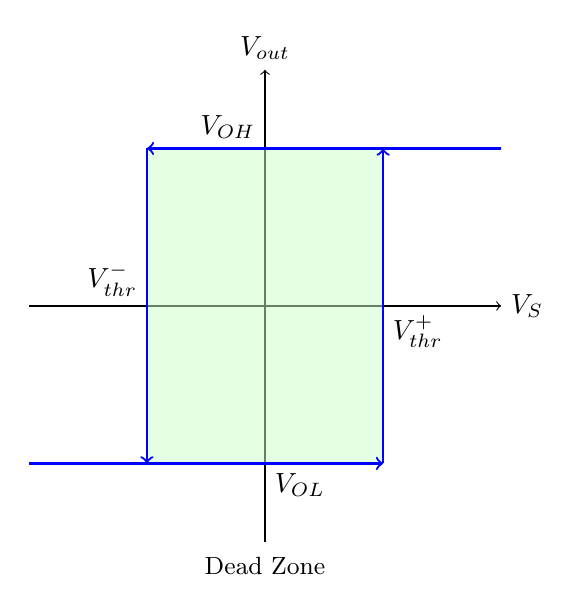
\begin{tikzpicture}
    \draw[->] (-3,0) -- (3,0) node[right] {$V_S$};
    \draw[->] (0,-3) -- (0,3) node[above] {$V_{\text{out}}$};
    \fill[green!20, opacity=0.5] (-1.5,-2) rectangle (1.5,2);
    \draw[thick, blue, arrows={->[scale=1.5]}] (3, 2) -- (-1.5, 2);
    \draw[thick, blue, arrows={->[scale=1.5]}] (-1.5, 2) -- (-1.5, -2);
    \draw[thick, blue, arrows={->[scale=1.5]}] (-3, -2) -- (1.5, -2);
    \draw[thick, blue, arrows={->[scale=1.5]}] (1.5, -2) -- (1.5, 2);
    \draw[thick, blue] (1.5, 2) -- (3, 2);
    \draw[thick, blue] (-1.5, -2) -- (-3, -2);
    \node[below right] at (1.5,0) {$V_{\text{thr}}^+$};
    \node[above left] at (-1.5,0) {$V_{\text{thr}}^-$};
    \node[above left] at (0,2) {$V_{OH}$};
    \node[below right] at (0,-2) {$V_{OL}$};
    \node at (0, -3.3) {\small Dead Zone};
\end{tikzpicture}
\end{fitcenter}

La zona verde è la \textbf{dead zone}: finché $V_S$ oscilla all'interno di $[V_{\text{thr}}^-, V_{\text{thr}}^+]$, l'uscita non commuta. Aumentando $R_2/R_1$ si restringe la zona morta (soglie più vicine a zero); diminuendo $R_2/R_1$ si allarga.

\subsection{Trigger di Schmitt invertente}

Nella versione invertente, il segnale $V_S$ è applicato al pin $-$ e il feedback positivo è portato sul pin $+$:

\begin{figure}[H]
\centering
\begin{circuitikz}[american, transform shape]
    \draw (0,0) node[op amp] (opamp) {};
    % Pin - (top): ingresso segnale VS
    \draw (opamp.-) to[short, -o] (-2.5, 0.5) node[left] {$V_S$};
    
    % Pin + (bottom): partitore
    \draw (opamp.+) -- (-1.2, -0.5);
    \fill (-1.2, -0.5) circle (2pt);
    
    % R1 verso ground (alzata per non toccare il ramo R2 sottostante)
    \draw (-1.2, -0.5) to[R, l=$R_1$] (-1.2, -1.7) node[ground] {};
    
    % Feedback R2 verso l'uscita (distanziato a y = -2.7)
    \draw (-1.2, -0.5) -- (-2.2, -0.5) -- (-2.2, -2.7) to[R, l=$R_2$] (1.5, -2.7) -- (1.5, 0);
    
    \fill (1.5, 0) circle (2pt);
    \draw (1.5, 0) -- (opamp.out);
    \draw (1.5, 0) to[short, -o] (2.5, 0) node[right] {$V_{\text{out}}$};
\end{circuitikz}
\caption{Trigger di Schmitt in configurazione invertente.}
\end{figure}

Ora $V_+ = \frac{R_1}{R_1+R_2} V_{\text{out}}$ e l'uscita commuta quando $V_S$ attraversa questo valore. Con uscita alta la soglia è $V_{\text{thr}}^+ = \frac{R_1}{R_1+R_2} V_{OH} > 0$: quando $V_S$ la supera l'uscita scende a $V_{OL}$. Con uscita bassa la soglia è $V_{\text{thr}}^- = \frac{R_1}{R_1+R_2} V_{OL} < 0$: quando $V_S$ scende sotto di essa l'uscita torna a $V_{OH}$. Il ciclo di isteresi è percorso in senso \textbf{orario}:

\begin{fitcenter}
\begin{tikzpicture}
    \draw[->] (-3,0) -- (3,0) node[right] {$V_S$};
    \draw[->] (0,-3) -- (0,3) node[above] {$V_{\text{out}}$};
    \draw[thick, blue, arrows={->[scale=1.5]}] (3, -2) -- (-1.5, -2);
    \draw[thick, blue, arrows={->[scale=1.5]}] (-1.5, -2) -- (-1.5, 2);
    \draw[thick, blue, arrows={->[scale=1.5]}] (-1.5, 2) -- (1.5, 2);
    \draw[thick, blue, arrows={->[scale=1.5]}] (1.5, 2) -- (1.5, -2);
    \draw[thick, blue] (1.5, -2) -- (3, -2);
    \draw[thick, blue] (-3, 2) -- (-1.5, 2);
    \draw[dashed] (1.5,0) node[above right] {$V_{\text{thr}}^+$} -- (1.5,2);
    \draw[dashed] (-1.5,0) node[below left] {$V_{\text{thr}}^-$} -- (-1.5,-2);
    \node[above left] at (0,2) {$V_{OH}$};
    \node[below right] at (0,-2) {$V_{OL}$};
    \begin{scope}[on background layer]
    \fill[green!20, opacity=0.5] (-1.5,-2) rectangle (1.5,2);
    \end{scope}
    \node at (0, -3.3) {\small Dead Zone};
\end{tikzpicture}
\end{fitcenter}

\begin{important}
\textbf{Confronto invertente / non invertente:}
\begin{itemize}
    \item \textbf{Non invertente}: il loop di isteresi è percorso in senso antiorario ($\circlearrowleft$); per $V_S$ molto grande l'uscita è alta.
    \item \textbf{Invertente}: il loop di isteresi è percorso in senso orario ($\circlearrowright$); per $V_S$ molto grande l'uscita è bassa.
    \item Le soglie del non invertente dipendono da $-R_1/R_2$; quelle dell'invertente da $R_1/(R_1+R_2)$. In entrambi i casi la soglia positiva è legata a un livello di uscita e quella negativa all'altro.
\end{itemize}
\end{important}

\section{Generatori di onde}

Un \textbf{generatore di onde} è una configurazione ad anello composta da un \textbf{Trigger di Schmitt} e un \textbf{circuito integratore} (con segno opposto al trigger). 

\begin{figure}[H]
\centering
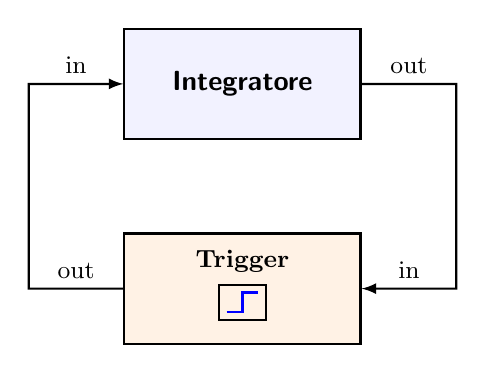
\begin{tikzpicture}[>=latex, font=\sffamily]
    % Integratore block
    \node[draw, thick, minimum width=3cm, minimum height=1.4cm, fill=blue!5] (int) at (0, 1.8) {\textbf{Integratore}};
    
    % Trigger block
    \node[draw, thick, minimum width=3cm, minimum height=1.4cm, fill=orange!10] (trig) at (0, -0.8) {};
    % Trigger label and hysteresis symbol inside
    \node[font=\small\bfseries] at (0, -0.45) {Trigger};
    \draw[thick] (-0.3, -1.2) rectangle (0.3, -0.75);
    \draw[thick, blue] (-0.2, -1.1) -- (0, -1.1) -- (0, -0.85) -- (0.2, -0.85);

    % Connections - Left (Trigger out -> Integratore in)
    \draw[->, thick] (trig.west) -- ++(-1.2,0) node[above, pos=0.5, font=\small] {out} 
                     -- ++(0, 2.6) 
                     -- (int.west) node[above, pos=0.5, font=\small] {in};
    
    % Connections - Right (Integratore out -> Trigger in)
    \draw[->, thick] (int.east) -- ++(1.2,0) node[above, pos=0.5, font=\small] {out} 
                     -- ++(0, -2.6) 
                     -- (trig.east) node[above, pos=0.5, font=\small] {in};
\end{tikzpicture}
\caption{Schema a blocchi di un generatore di onde.}
\end{figure}

L'uscita del trigger non è mai stabile: commuta periodicamente fra le due saturazioni a causa dell'anello. Si ha quindi la produzione di:
\[
    \begin{cases}
        \text{onda quadra} & \text{all'uscita del Trigger} \\[0.3em]
        \text{onda triangolare} & \text{all'uscita dell'integratore}
    \end{cases}
\]

\subsection{Multivibratore astabile}

Un classico esempio è il \textbf{multivibratore astabile} a singolo amplificatore operazionale. In questo circuito, l'operazionale funge da comparatore con isteresi (grazie alla retroazione positiva tramite $R_1$ e $R_2$), mentre la rete $RC$ (retroazione negativa) funge da integratore passivo che genera l'andamento esponenziale del segnale.

\begin{figure}[H]
\centering
\begin{circuitikz}[american, transform shape]

    % Op-amp centrale
    \draw (0,0) node[op amp] (opamp) {};

    % Uscita e terminale out_trig
    \draw (opamp.out) -- (2,0);
    \fill (2,0) circle (2pt);
    \draw (2,0) to[short, -o] (2.8,0) node[right] {$\text{out}_{\text{trig}}$};

    % Retroazione negativa: resistenza R in alto
    \draw (opamp.-) -- (-1.2, 1.8) to[R, l=$R$] (2, 1.8) -- (2,0);

    % Partitore R2-R1 a destra per la retroazione positiva
    \draw (2,0) to[R, l=$R_2$] (2, -1.5) coordinate (divider) to[R, l=$R_1$] (2, -3) node[ground] {};
    \fill (divider) circle (2pt);
    \draw (divider) -- (-1.2, -1.5) -- (opamp.+);

    % Ingresso invertente: Condensatore C a massa e terminale out_integr
    \fill (opamp.-) circle (2pt);
    \draw (opamp.-) -- (-2.2, 0.5);
    \fill (-2.2, 0.5) circle (2pt);
    \draw (-2.2, 0.5) to[C, l=$C$] (-2.2, -1.8) node[ground] {};
    \draw (-2.2, 0.5) to[short, -o] (-3.2, 0.5) node[left] {$\text{out}_{\text{integr}}$};

\end{circuitikz}
\caption{Circuito del multivibratore astabile a singolo operazionale.}
\end{figure}

\textbf{Analisi del funzionamento.} Supponiamo che all'istante $t=0$ l'uscita del Trigger sia $V_{\text{out,trig}} = V_{OH}$. Il condensatore inizia a caricarsi (o scaricarsi) attraverso $R$ verso $V_{OH}$ (o $V_{OL}$) con costante di tempo $\tau = RC$, descrivendo un transitorio esponenziale. Questa rampa viene riportata all'ingresso $V_-$ del Trigger.

Il Trigger commuta quando $V_- = V_+ = \frac{R_1}{R_1+R_2} V_{OH} \equiv V_{\text{thr}}^+$. La tensione $V_-(t)$ segue il transitorio RC verso l'asintotico $V_{OH}$, partendo da $V_{\text{thr}}^- = \frac{R_1}{R_1+R_2} V_{OL}$:
\[
    V_-(t) = V_{OH} + \left(\frac{R_1}{R_1+R_2} V_{OL} - V_{OH}\right) e^{-t/\tau}
\]

\textbf{Calcolo di $T_H$.} Imponendo $V_-(T_H) = V_{\text{thr}}^+ = \frac{R_1}{R_1+R_2} V_{OH}$:
\[
    \frac{R_1}{R_1+R_2} V_{OH} = V_{OH} + \left(\frac{R_1}{R_1+R_2} V_{OL} - V_{OH}\right) e^{-T_H/\tau}
\]
Raccogliendo e risolvendo per $T_H$:
\[
    e^{-T_H/\tau} = \frac{\frac{R_1}{R_1+R_2} V_{OH} - V_{OH}}{\frac{R_1}{R_1+R_2} V_{OL} - V_{OH}}
    = \frac{-\frac{R_2}{R_1+R_2} V_{OH}}{\frac{R_1}{R_1+R_2} V_{OL} - V_{OH}}
\]
\[
    \boxed{T_H = RC \ln \left[ 1 + \frac{R_1}{R_2} \left( 1 - \frac{V_{OL}}{V_{OH}} \right) \right]}
    \xrightarrow{V_{OL} = -V_{OH}} RC \ln\!\left(1 + 2\frac{R_1}{R_2}\right)
\]

\textbf{Calcolo di $T_L$.} Per simmetria, scambiando $V_{OH} \leftrightarrow V_{OL}$:
\[
    \boxed{T_L = RC \ln \left[ 1 + \frac{R_1}{R_2} \left( 1 - \frac{V_{OH}}{V_{OL}} \right) \right]}
    \xrightarrow{V_{OL} = -V_{OH}} RC \ln\!\left(1 + 2\frac{R_1}{R_2}\right)
\]

Con livelli simmetrici $V_{OH} = -V_{OL} = V_{\text{sat}}$, risulta $T_H = T_L$ e il \textbf{periodo totale} è:
\[
    T = T_H + T_L = 2RC\ln\!\left(1 + 2\frac{R_1}{R_2}\right)
    \qquad \text{duty cycle} = 50\%
\]

\begin{figure}[H]
\centering
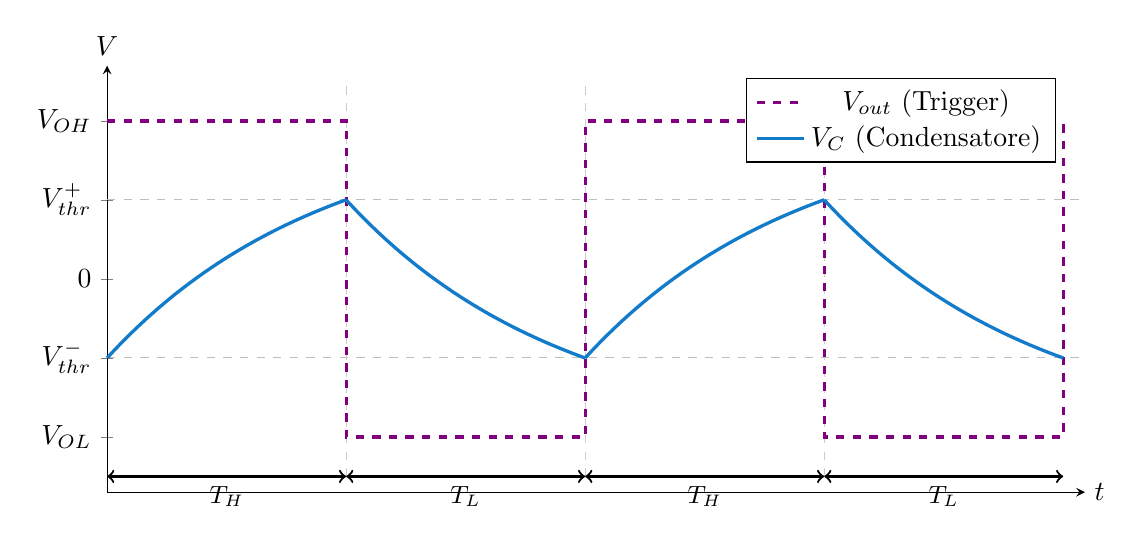
\begin{tikzpicture}
\begin{axis}[
    width=14cm, height=7cm,
    axis lines=left,
    xlabel={$t$},
    ylabel={$V$},
    xmin=0, xmax=4.5,
    ymin=-2.7, ymax=2.7,
    xtick=\empty,
    ytick={-2,-1,0,1,2},
    yticklabels={$V_{OL}$, $V_{\text{thr}}^-$, $0$, $V_{\text{thr}}^+$, $V_{OH}$},
    every axis x label/.style={at={(ticklabel* cs:1)},anchor=west},
    every axis y label/.style={at={(ticklabel* cs:1)},anchor=south},
    legend pos=north east,
    clip=false,
]
% --- Linee guida soglie ---
\addplot[gray!50, thin, dashed, forget plot] coordinates {(0,1) (4.5,1)};
\addplot[gray!50, thin, dashed, forget plot] coordinates {(0,-1) (4.5,-1)};

% --- Linee verticali agli istanti di commutazione ---
% TH1 termina a t=1.1, TL1 termina a t=2.2, TH2 termina a t=3.3, TL2 termina a t=4.4
\draw[gray!40, thin, dashed] (axis cs:1.1, -2.5) -- (axis cs:1.1, 2.5);
\draw[gray!40, thin, dashed] (axis cs:2.2, -2.5) -- (axis cs:2.2, 2.5);
\draw[gray!40, thin, dashed] (axis cs:3.3, -2.5) -- (axis cs:3.3, 2.5);

% --- Onda quadra Trigger (viola, tratteggiato) ---
% Parte a VOH=2, scende a VOL=-2 a t=1.1, torna su a t=2.2, ecc.
\addplot[violet, very thick, dashed, const plot, mark=none] coordinates {
    (0,2) (1.1,-2) (2.2,2) (3.3,-2) (4.4,2)
};
\addlegendentry{$V_{\text{out}}$ (Trigger)}

% --- Tensione sul condensatore Vc (azzurro, solido) ---
% t in [0, 1.1]: trigger=+2, Vc sale da Vthr-=-1 verso asintotico VOH=+2: Vc = 2 - 3*exp(-t/tau)
% (scatta quando Vc = Vthr+ = +1, cioè quando 2-3exp(-t/tau)=1 => exp = 1/3 => t=tau*ln3 = 1.1 con tau=1)
\addplot[cyan!60!blue, very thick, domain=0:1.1, samples=80] {2 - 3*exp(-x)};
% t in [1.1, 2.2]: trigger=-2, Vc scende da Vthr+=+1 verso VOL=-2: Vc = -2 + 3*exp(-(t-1.1)/tau)
\addplot[cyan!60!blue, very thick, domain=1.1:2.2, samples=80] {-2 + 3*exp(-(x-1.1))};
% t in [2.2, 3.3]: trigger=+2, sale
\addplot[cyan!60!blue, very thick, domain=2.2:3.3, samples=80] {2 - 3*exp(-(x-2.2))};
% t in [3.3, 4.4]: trigger=-2, scende
\addplot[cyan!60!blue, very thick, domain=3.3:4.4, samples=80] {-2 + 3*exp(-(x-3.3))};
\addlegendentry{$V_C$ (Condensatore)}

% --- Frecce doppie TH / TL ---
\draw[<->, thick] (axis cs:0,   -2.5) -- node[below, font=\small] {$T_H$} (axis cs:1.1, -2.5);
\draw[<->, thick] (axis cs:1.1, -2.5) -- node[below, font=\small] {$T_L$} (axis cs:2.2, -2.5);
\draw[<->, thick] (axis cs:2.2, -2.5) -- node[below, font=\small] {$T_H$} (axis cs:3.3, -2.5);
\draw[<->, thick] (axis cs:3.3, -2.5) -- node[below, font=\small] {$T_L$} (axis cs:4.4, -2.5);

\end{axis}
\end{tikzpicture}
\caption{Forme d'onda del multivibratore astabile: \textbf{onda quadra} (viola tratteggiata) all'uscita
del Trigger e \textbf{tensione sul condensatore} $V_C$ (azzurro) con andamento esponenziale tra
$V_{\text{thr}}^+$ e $V_{\text{thr}}^-$. Le commutazioni avvengono esattamente quando $V_C$
tocca la soglia corrispondente.}
\end{figure}

\textbf{Lettura del grafico.}
\begin{itemize}
    \item Nel semi-periodo $T_H$ (trigger a $V_{OH}$): il condensatore si carica attraverso $R$, quindi $V_C$ \emph{cresce esponenzialmente} verso $V_{OH}$ partendo da $V_{\text{thr}}^-$; quando raggiunge la soglia superiore $V_{\text{thr}}^+$, il trigger commuta a $V_{OL}$.
    \item Nel semi-periodo $T_L$ (trigger a $V_{OL}$): $V_C$ \emph{decresce esponenzialmente} verso $V_{OL}$; quando raggiunge $V_{\text{thr}}^-$, il trigger commuta nuovamente a $V_{OH}$.
    \item Con $V_{OH} = -V_{OL}$ e $R_1, R_2$ fissati, si ha $T_H = T_L$ e il segnale quadro ha duty cycle del $50\%$.
\end{itemize}

\subsection{Circuito con integratore di Miller (a due operazionali)}

Un'ulteriore configurazione fondamentale per la generazione di forme d'onda è il circuito a due operazionali, composto da un \textbf{Trigger di Schmitt non invertente} e un \textbf{integratore di Miller} attivo. A differenza del multivibratore a singolo op-amp con rete RC passiva, l'utilizzo dell'integratore di Miller consente di ottenere rampe perfettamente lineari all'uscita dell'integratore (onda triangolare pura) anziché andamenti esponenziali.

\begin{figure}[H]
\centering
\begin{circuitikz}[american, transform shape]

    % === Op-Amp 1: Trigger di Schmitt Non Invertente ===
    \draw (0,0) node[op amp, noinv input up] (op1) {};
    \node[font=\small, above] at (0, 0.8) {Trigger};

    % Pin - del Trigger (in basso): a massa
    \draw (op1.-) -- (-1.2, -0.5) -- (-1.2, -1.5) node[ground] {};

    % Pin + del Trigger (in alto): giunzione R1 e R2
    \coordinate (nodeplus) at (-1.2, 0.5);
    \draw (op1.+) -- (nodeplus);
    \fill (nodeplus) circle (2pt);

    % Resistenza R1 dall'ingresso in_trig (uscita integratore) al Pin +
    \draw (nodeplus) to[R, l_=$R_1$, -o] (-3.5, 0.5) node[left] {$\text{in}_{\text{trig}}$};

    % Uscita Op1 (out_trig)
    \coordinate (outtrig) at (1.8, 0);
    \draw (op1.out) -- (outtrig);
    \fill (outtrig) circle (2pt);
    \draw (outtrig) to[short, -o] (1.8, -1.2) node[below] {$\text{out}_{\text{trig}}$};

    % Resistenza R2 di retroazione positiva dal nodo outtrig al Pin +
    \draw (nodeplus) -- (-1.2, 1.8) to[R, l=$R_2$] (1.8, 1.8) -- (outtrig);

    % === Op-Amp 2: Integratore di Miller ===
    \draw (5.5, 0) node[op amp] (op2) {};
    \node[font=\small, above] at (5.5, 0.8) {Integratore};

    % Pin + dell'Integratore (in basso): a massa
    \draw (op2.+) -- (4.3, -0.5) -- (4.3, -1.5) node[ground] {};

    % Pin - dell'Integratore (in alto): giunzione per R e C
    \coordinate (nodeminus) at (4.3, 0.5);
    \draw (op2.-) -- (nodeminus);
    \fill (nodeminus) circle (2pt);

    % Resistenza R da outtrig (uscita Trigger) al Pin - dell'Integratore
    \draw (outtrig) to[R, l=$R$] (nodeminus);

    % Condensatore C in retroazione (da outinteg a Pin -)
    \coordinate (outinteg) at (7.2, 0);
    \draw (op2.out) -- (outinteg);
    \fill (outinteg) circle (2pt);
    \draw (outinteg) to[short, -o] (8.2, 0) node[right] {$\text{out}_{\text{integ}}$};

    \draw (nodeminus) -- (4.3, 1.8) to[C, l=$C$] (7.2, 1.8) -- (outinteg);

    % === Anello di retroazione: da out_integ a in_trig ===
    \draw (outinteg) -- (7.2, 2.7) -- (-3.5, 2.7) -- (-3.5, 0.5);

\end{circuitikz}
\caption{Circuito generatore di forme d'onda a due operazionali con integratore di Miller.}
\end{figure}

\noindent\textbf{Funzionamento.} Siano $V_{OH} = -V_{OL} = V_{\text{sat}}$.
\begin{itemize}
    \item Il trigger è non invertente con ingresso $\text{in}_{\text{trig}} = \text{out}_{\text{integ}}$: le sue soglie sono $V_{\text{thr}}^\pm = \pm\frac{R_1}{R_2}V_{\text{sat}}$.
    \item Quando l'uscita del trigger vale $+V_{\text{sat}}$, l'integratore invertente produce una rampa \textbf{decrescente} con pendenza costante $-\frac{V_{\text{sat}}}{RC}$; quando la rampa raggiunge $V_{\text{thr}}^-$ il trigger commuta a $-V_{\text{sat}}$ e la rampa diventa \textbf{crescente} con pendenza $+\frac{V_{\text{sat}}}{RC}$, fino a $V_{\text{thr}}^+$.
    \item L'uscita dell'integratore è quindi un'\textbf{onda triangolare} di ampiezza picco-picco $2\frac{R_1}{R_2}V_{\text{sat}}$, quella del trigger un'\textbf{onda quadra} di ampiezza $\pm V_{\text{sat}}$.
\end{itemize}
Ogni rampa deve percorrere $\Delta V = 2\frac{R_1}{R_2}V_{\text{sat}}$ con pendenza $\frac{V_{\text{sat}}}{RC}$, quindi dura $T/2 = 2RC\frac{R_1}{R_2}$ e il periodo vale:
\[
    T = 4RC\,\frac{R_1}{R_2}
\]
Per avere oscillazione le soglie devono essere minori della saturazione, cioè $R_1 < R_2$.

\section*{Riepilogo del Capitolo}

\begin{important}
Le applicazioni non lineari degli Op-Amp sfruttano il \textbf{feedback positivo}: l'uscita satura a $V_{OH}$ o $V_{OL}$ e non esiste un punto di lavoro lineare stabile.
\end{important}

\begin{note}
\textbf{Trigger di Schmitt — regole pratiche:}
\begin{itemize}
    \item \textbf{Non invertente}: soglie $V_{\text{thr}}^+ = -\dfrac{R_1}{R_2} V_{OL}$, $V_{\text{thr}}^- = -\dfrac{R_1}{R_2} V_{OH}$, loop antiorario.
    \item \textbf{Invertente}: soglie $V_{\text{thr}}^+ = \dfrac{R_1}{R_1+R_2} V_{OH}$, $V_{\text{thr}}^- = \dfrac{R_1}{R_1+R_2} V_{OL}$, loop orario.
    \item La \textbf{dead zone} $[V_{\text{thr}}^-, V_{\text{thr}}^+]$ determina l'immunità al rumore.
    \item \textbf{Multivibratore astabile} con $V_{OH} = -V_{OL}$: periodo $T = 2RC\ln\!\left(1 + 2\dfrac{R_1}{R_2}\right)$.
    \item \textbf{Generatore con integratore di Miller}: onda triangolare lineare, periodo $T = 4RC\dfrac{R_1}{R_2}$.
\end{itemize}
\end{note}


